\begin{figure*}[!hbtp]
  \centering

  \subfloat{
    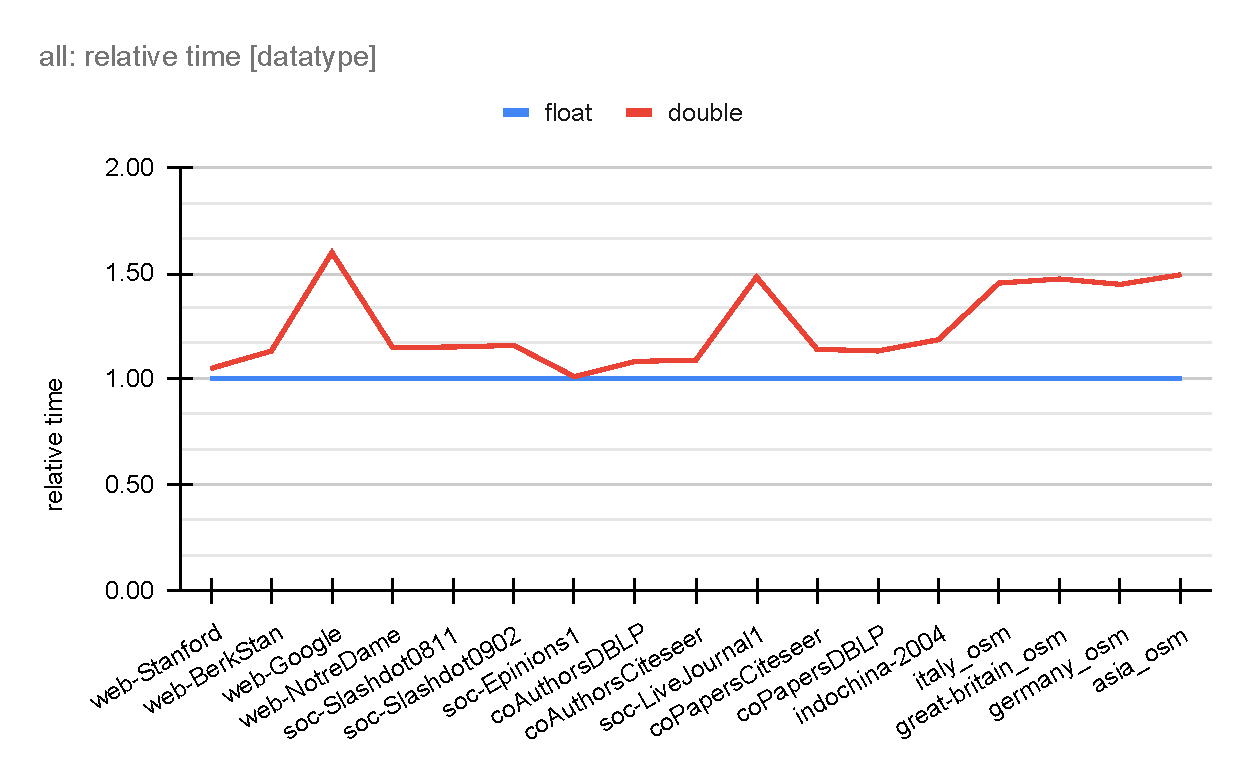
\includegraphics[width=0.48\textwidth]{out/pr-cuda-adj-rtype-rtime.pdf}
    \label{fig:pr-cuda-adj-rtype-rtime}
  }
  \subfloat{
    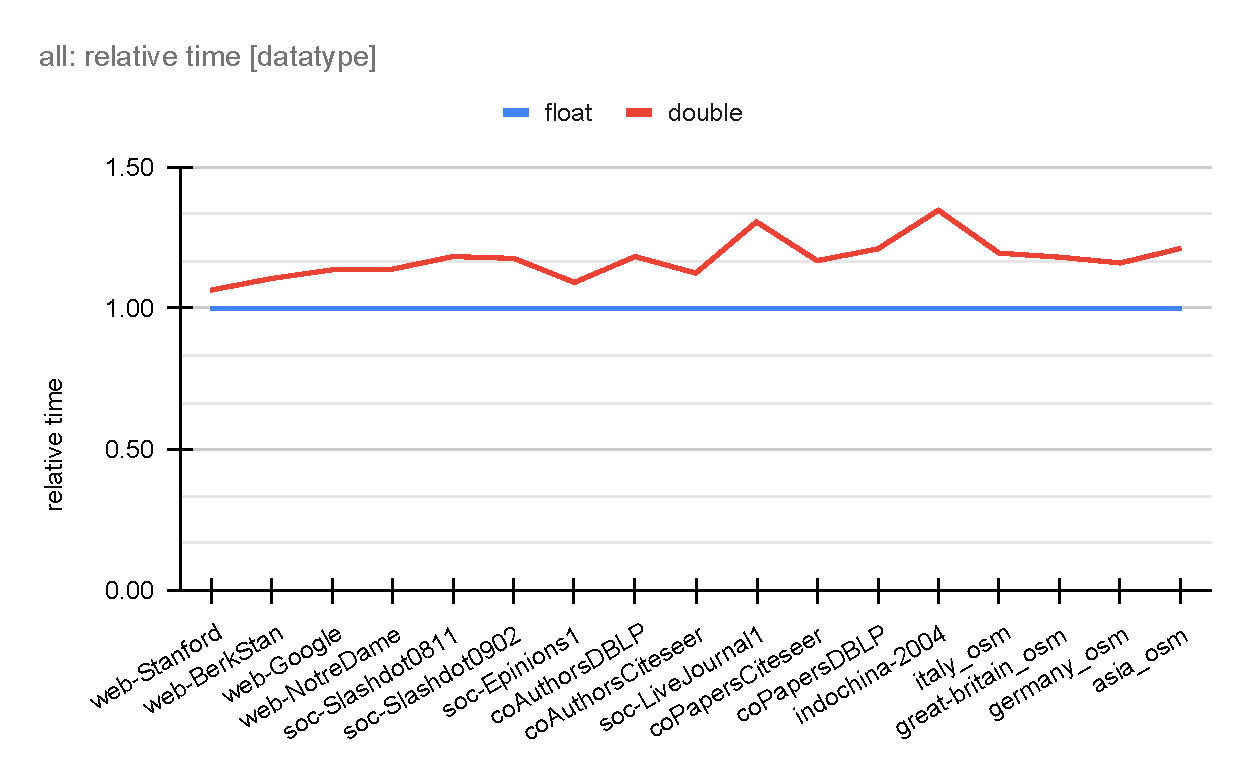
\includegraphics[width=0.48\textwidth]{out/pr-cuda-adj-ctype-rtime.pdf}
    \label{fig:pr-cuda-adj-ctype-rtime}
  }

  \caption{Relative time taken for switched thread/block-per-vertex CUDA-based (GPU) PageRank computation with the following datatypes for the rank vector is shown on the left: 32-bit floating point (float), 64-bit floating point (double). Relative time taken for CSR representation with the following datatypes is shown on the right: 32-bit integer (int32), 64-bit integer (int64). This is done on 5 web graphs, 4 social networks, 4 collaboration networks, and 4 road networks.}
  \label{fig:pr-cuda-adj-type}
\end{figure*}
